%!TEX root = ../dissertation.tex

\graphicspath{{4-methods/figures/}}
\chapter{Methodology and Challenges}
\label{ch:methods}

The chapter outlines the prospective methodologies for this thesis and discusses the expected challenges in the proposed research directions.
It is unavoidable that the content of this chapter includes a certain degree of abstractness and ambiguity, because, as in most machine learning research, there is no predefined protocol for performing the research, and the very goal of this study lies on finding a methodology that works.
In light of this, the following section illustrates the high-level ideas, and the perspectives on generative models and the concept of disentanglement are presented, followed by the description of the datasets to be used in the research.


\section{The High-Level Ideas}

\begin{figure}
	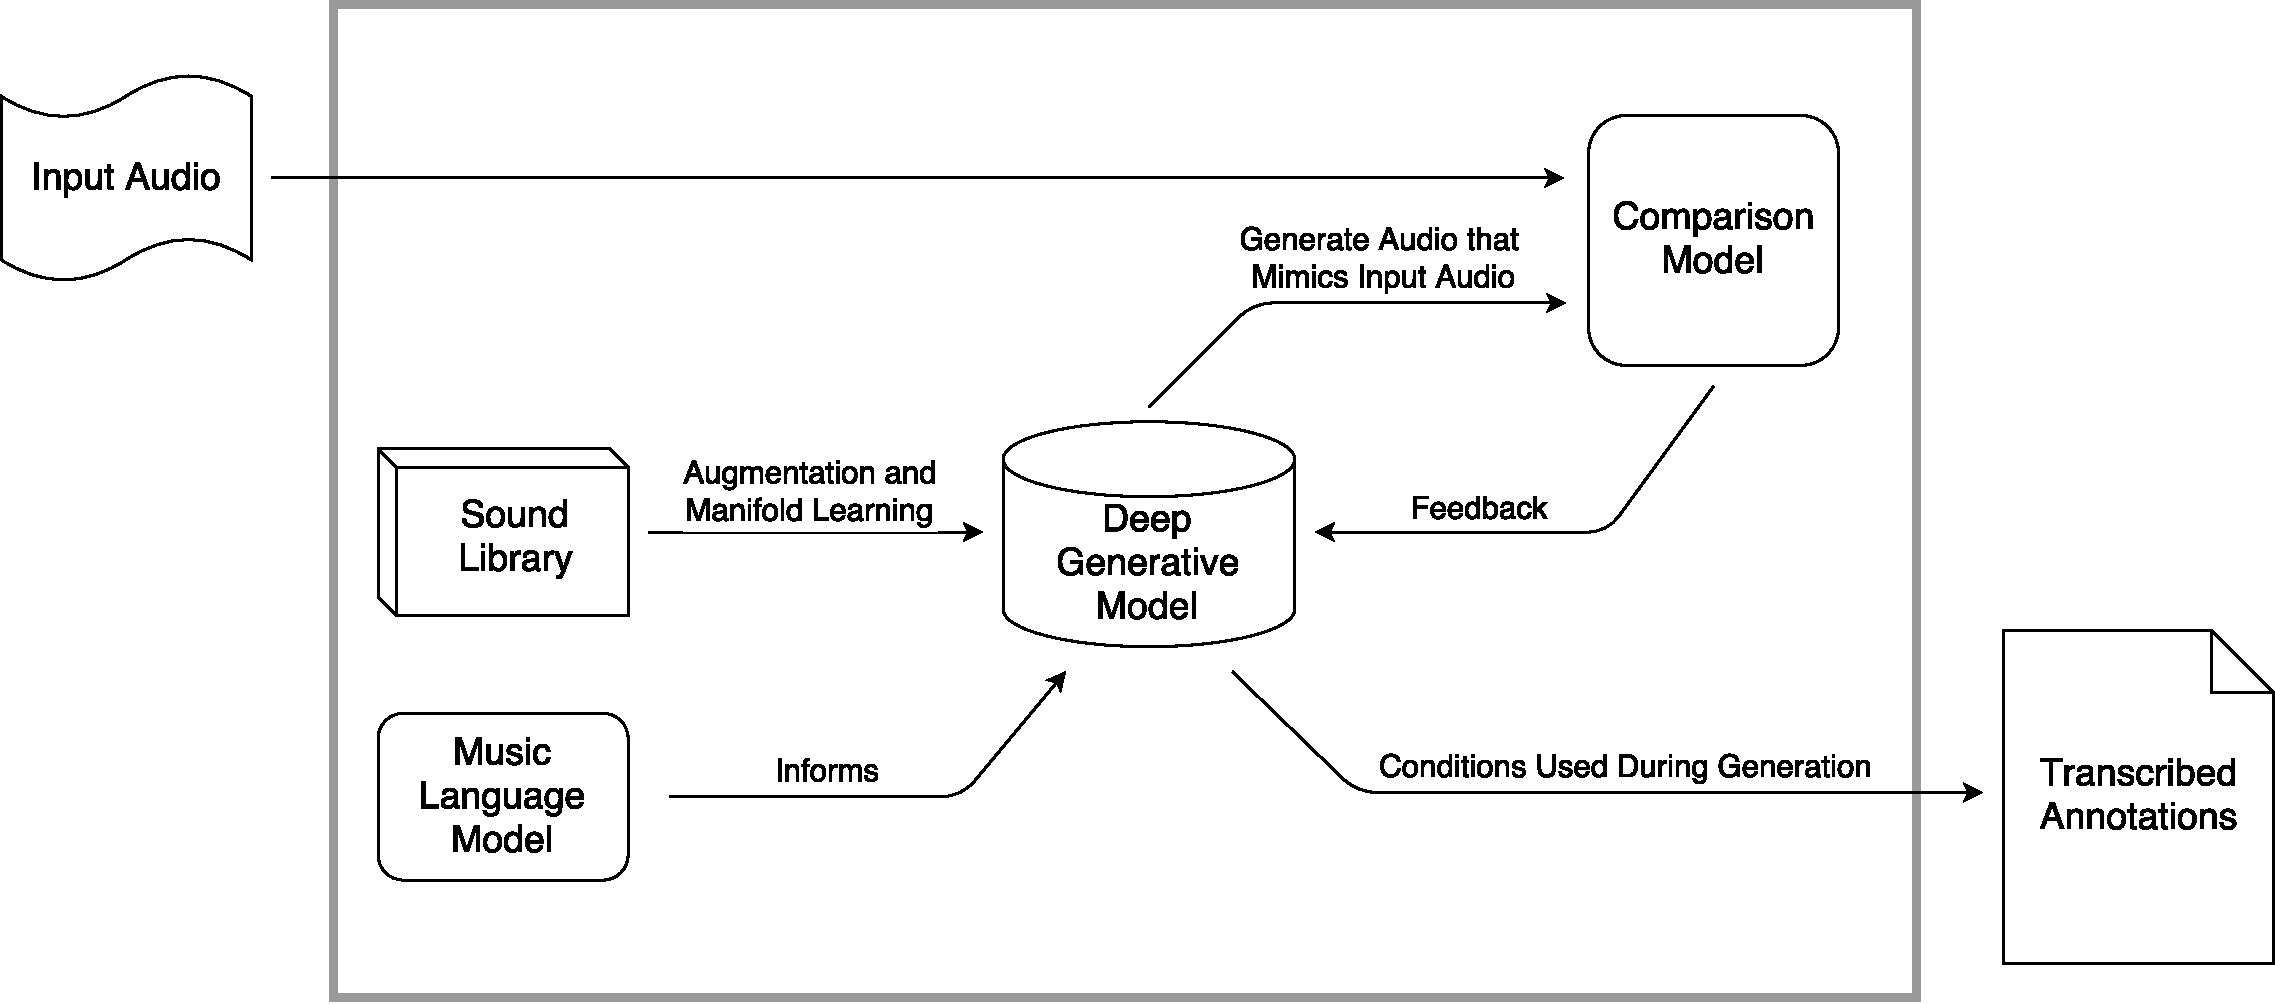
\includegraphics[width=\textwidth]{grand.pdf}
	\caption{A high-level schematic of the proposed automatic music transcription system. A deep generative model is trained using music database and music language models, to generate audio track that sounds similarly as the input audio. The conditions used to generate the matching audio can produce the predicted music transcription. }\label{fig:grand}
\end{figure}

Figure \ref{fig:grand} shows the high-level diagram for an end-to-end automatic music transcription system built around a deep generative model.
In short, the deep generative model in the center will learn to generate audio signals that mimics the input, and the combinations of instruments and pitches used for generating the audio will be the resulting transcription.
In order for the generative model to learn the semantic latent variables in music, the model needs to be able to disentangle the pitch and timbre information from the audio.
While the techniques such as batch normalization and using diagonal covariance matrices in variational autoencoders are intended to induce statistical independence between latent components,
making the components have a fully disentangled semantic information remains an active area of research.
The next section discusses the possible methods for disentanglement in the context of deep generative models.

The proposed transcription system is not only powered by deep generative models and music language models, but also by a few other important techniques that will make the implementation possible to be realized.
Data augmentation is a method for increasing the quantity of available data using transformations that does not alter or deterministically alter the label, and has been successfully applied to image classification tasks  \cite{krizhevsky2012imagenet}. MUDA \cite{mcfee2015muda} provides a software framework for augmenting musical audio, which supports pitch shift, time stretch, background noise, and dynamic range compression.
It would be also possible augment the data by filtering with the impulse responses according to various room acoustics, adding reverberations to the audio.
Combined with the audio sources from various software instruments and sample libraries, these methods for audio augmentation can greatly increase the effective size of training data, and will help the deep model to more accurately learn the distribution of the real-world musical sounds.
It is more efficient in terms of both time and space complexity to perform data augmentation on-the-fly instead of storing precomputed data, because the size of data increases combinatorially depending on the available augmentation schemes.


\section{Generative Models and Learning Disentangled Representations}

\TODO{section outline:}

\begin{itemize}
	\item revisit the definition of generative model
	\item we will use a relaxed definition for the term `generative':
	\item distinguish data and label as:
	\begin{itemize}
		\item data: high-dimensional, observed raw, entangled information
		\item label: low-dimensional, often requiring manual annotations, disentangled information
	\end{itemize}
	\item representation learning and manifold learning
	\item what we need is: disentanglement
	\begin{itemize}
		\item literature review on disentanglement:
		\item \cite{brahma2016disentanglement}
		\item PCA, ICA, Matrix Factorization, etc.
		\item \cite{chen2016infogan}, \cite{achille2018information}, \cite{donahue2017gan}
	\end{itemize}
	\item why generative models are suitable for this
	\item planned strategies
	\begin{itemize}
		\item \cite{ganin2015domain}
		\item \cite{donahue2017gan}
	\end{itemize}
	\item expected challenges
	\begin{itemize}
		\item data dimension
		\item flood of GAN models
	\end{itemize}
\end{itemize}


\section{Methods}

\subsection{End-to-End Generative Model between Audio and Piano Rolls}

\paragraph{Disentangling Pitch and Timbre}

\paragraph{Extending to Variable Time Scale}

\paragraph{Obtaining Piano Rolls}

\subsection{Generative Model as Augmentation}

\paragraph{Software Instrument and Audio Post-Processing}

\paragraph{Toward Better Music Language Models}

\paragraph{Positive Feedback Cycle between Transcription and Augmentation}


\section{Datasets}

The experiments are based on a few publicly and commercially available datasets including RWC Music Database \cite{goto2003rwc}, MedleyDB \cite{bittner2014medleydb}, and Vienna Symphonic Library of orchestral sounds as studied in \cite{humphrey2011nlse}.
In future studies, the NSynth Dataset published recently by Google's Magenta project \cite{engel2017nsynth} is also planned to be used, as the dataset contains additional kinds of instruments and comes with more accurate annotations.

\TODO{NSynth, Vienna Symphonic, Logic Pro with Audio Units}
\TODO{Add MusicNet, Bach10, SU, Weimar Jazz dataset for benchmark, show statistics; possibility of using proprietary software instruments like in Logic Pro; symbolic music datasets; with references}
